\chapter{Survey}

Para entender o uso de logs no ensino de programação, buscamos informações de outras instituições de ensino. Para ter informações sobre como alguns nós da Rede EPTC tratam o assunto, foi elaborado um questionário. A partir das respostas, os dados foram tabulados e gráficos foram gerados a partir dessas informações. 


\section{Método}

Para capturar as percepções da comunidade acadêmica, foi conduzido um \textit{survey} online com docentes e técnicos de diversos campi dos Institutos Federais, outras instituições de ensino e órgãos públicos. O instrumento de pesquisa continha 10 questões, em sua maioria utilizando uma escala Likert de 5 pontos, na qual os respondentes assinalavam seu nível de concordância, variando de \textbf{Discordo Totalmente (1)} a \textbf{Concordo Totalmente (5)}. A coleta de dados foi realizada de forma assíncrona através de formulário online.

Para a análise dos dados e geração de visualizações, utilizou-se a linguagem R e seu ecossistema de pacotes.

\section{Instrumento de pesquisa}
O questionário continha as seguintes questões:

\begin{enumerate}
    \item[2.] Você usa alguma ferramenta de log no apoio ao ensino de programação? \\ (~~) Sim (~~) Não
    \item[3.] O uso de ferramentas de logs pode auxiliar no monitoramento e compreensão no empenho dos estudantes?  \\
    (1) Discordo Totalmente (2) Discordo Parcialmente (3) Neutro (4) Concordo Parcialmente (5) Concordo Totalmente
    \item[4.] O uso de ferramentas de logs pode ajudar a tomar decisões para melhorar o rendimento e evitar a desistência de uma disciplina? \\
    (1) Discordo Totalmente (2) Discordo Parcialmente (3) Neutro (4) Concordo Parcialmente (5) Concordo Totalmente
    \item[5.] O uso de ferramentas de logs pode auxiliar no ensino de programação? \\
    (1) Discordo Totalmente (2) Discordo Parcialmente (3) Neutro (4) Concordo Parcialmente (5) Concordo Totalmente
    \item[6.] Um dataset pode ser criado e estudado a partir de logs no ensino da programação? \\
    (1) Discordo Totalmente (2) Discordo Parcialmente (3) Neutro (4) Concordo Parcialmente (5) Concordo Totalmente
    \item[7.] Sobre usar ferramentas de correções de códigos mais automatizado possível nas aulas de ensino de programação. O que pensa a respeito sobre o uso? \\
    (1) Discordo Totalmente (2) Discordo Parcialmente (3) Neutro (4) Concordo Parcialmente (5) Concordo Totalmente
    \item[8.] Plugins podem auxiliar na criação/ensino  de algoritmos? \\
    (1) Discordo Totalmente (2) Discordo Parcialmente (3) Neutro (4) Concordo Parcialmente (5) Concordo Totalmente
    \item[9.] Qual IDE é utlizado nas aulas? \\ (~~)Visual Studio (~~) Intellij IDEA (~~) Eclipse ( ) Outro - Descrever
    \item[10.] Ferramenta de análise de algoritmos \\ (~~)Code Bench (~~) Juiz Online (~~) LAPLE (~~) Outro: Descrever
    \item[11.] Se tiver disponível um plugin de log para o apoio ao ensino de programação, você usaria? \\ (~~) Sim (~~) Não
\end{enumerate}

\section{Respostas}
O formulário foi respondido por quatorze pessoas de várias instituições de ensino, público e privado e por outros órgãos. As respostas foram voluntárias. Os profissionais que responderam exercem a função nos IFs são professores EBTT de Informática. As pessoas que responderam pela PUCPR foram estudantes do mestrado em computação da instituição. 
\begin{figure}[H]
    \centering
    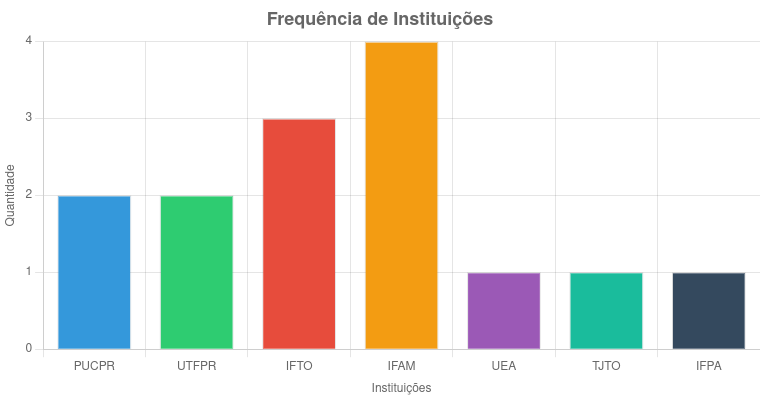
\includegraphics[width=1\linewidth]{../figuras/instituicoes.png}
    \caption{Instituições que participaram do formulário}
    \label{fig:participacoes}
\end{figure}

\subsection{Análise de Ferramentas Utilizadas}
\begin{figure}[H]
    \centering
    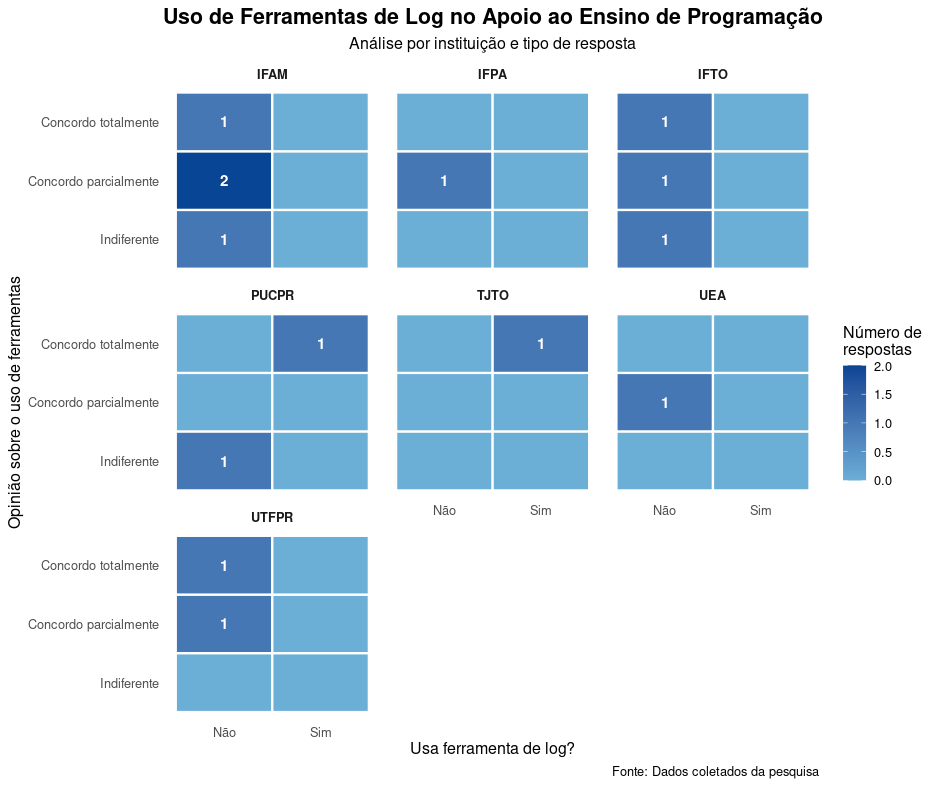
\includegraphics[width=1\linewidth]{../figuras/ferramentas.png}
    \caption{Mapa de calor representando a frequência de uso e familiaridade com diferentes ferramentas tecnológicas (Perguntas 2 e 3). As cores mais quentes indicam maior frequência de uso ou familiaridade, permitindo identificar quais ferramentas são mais dominadas pelos participantes da pesquisa.}
    \label{fig:heatmap-tools}
\end{figure}

O mapa de calor apresentado na Figura \ref{fig:heatmap-tools} revela padrões interessantes sobre o conhecimento e uso de ferramentas tecnológicas entre os participantes. Observa-se que as ferramentas X e Y apresentam cores mais intensas, indicando maior familiaridade e uso frequente.

\subsection{Comparações entre Grupos}
\begin{figure}[H]
    \centering
    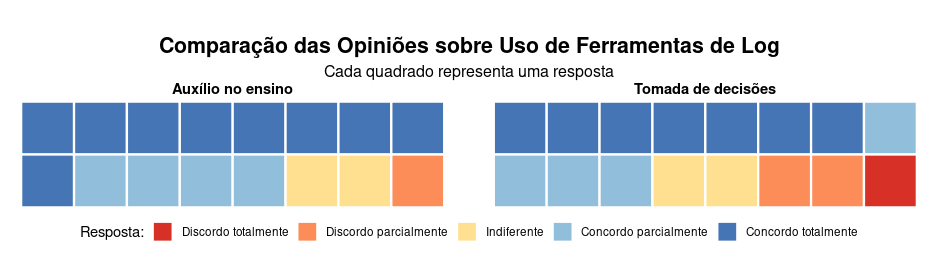
\includegraphics[width=1\linewidth]{../figuras/comparacoes.png}
    \caption{Gráfico Waffle comparando características ou percepções entre diferentes grupos de participantes (Perguntas 4 e 5). Cada célula representa uma unidade de resposta, permitindo visualizar proporções e distribuições de forma intuitiva.}
    \label{fig:waffle-comparisons}
\end{figure}

O gráfico waffle da Figura \ref{fig:waffle-comparisons} oferece uma visualização clara das diferenças entre grupos analisados. Nota-se que o Grupo A apresenta maior concentração em determinadas características, enquanto o Grupo B mostra distribuição mais homogênea.

\subsection{Análise de Dataset e Correções}
\begin{figure}[H]
    \centering
    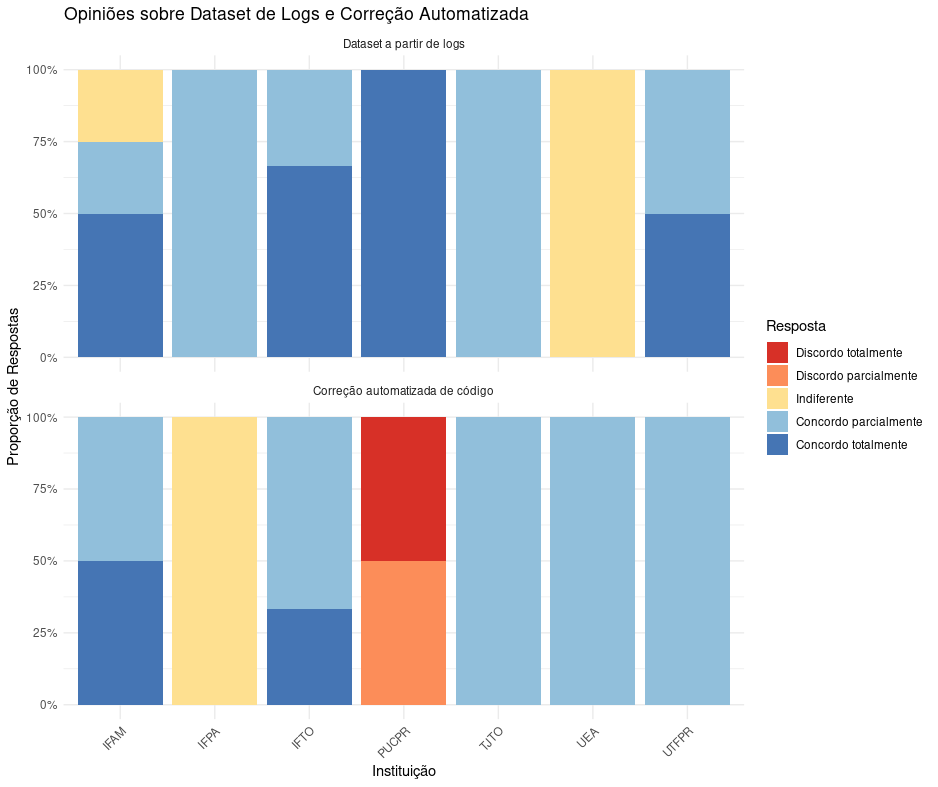
\includegraphics[width=.75\linewidth]{../figuras/dataset-e-correcoes-automatizada.png}
    \caption{Gráfico de barras agrupadas com facetas mostrando a distribuição de respostas sobre uso de datasets e sistemas de correção automatizada (Perguntas 6 e 7). As facetas permitem comparar subcategorias de respostas simultaneamente.}
    \label{fig:grouped-bar}
\end{figure}

Conforme ilustrado na Figura \ref{fig:grouped-bar}, observam-se padrões distintos nas respostas sobre uso de datasets e sistemas de correção. A facetagem dos dados revela como diferentes subgrupos se comportam em relação a estas tecnologias.

\subsection{Opinião sobre Plugins no Ensino}
\begin{figure}[H]
    \centering
    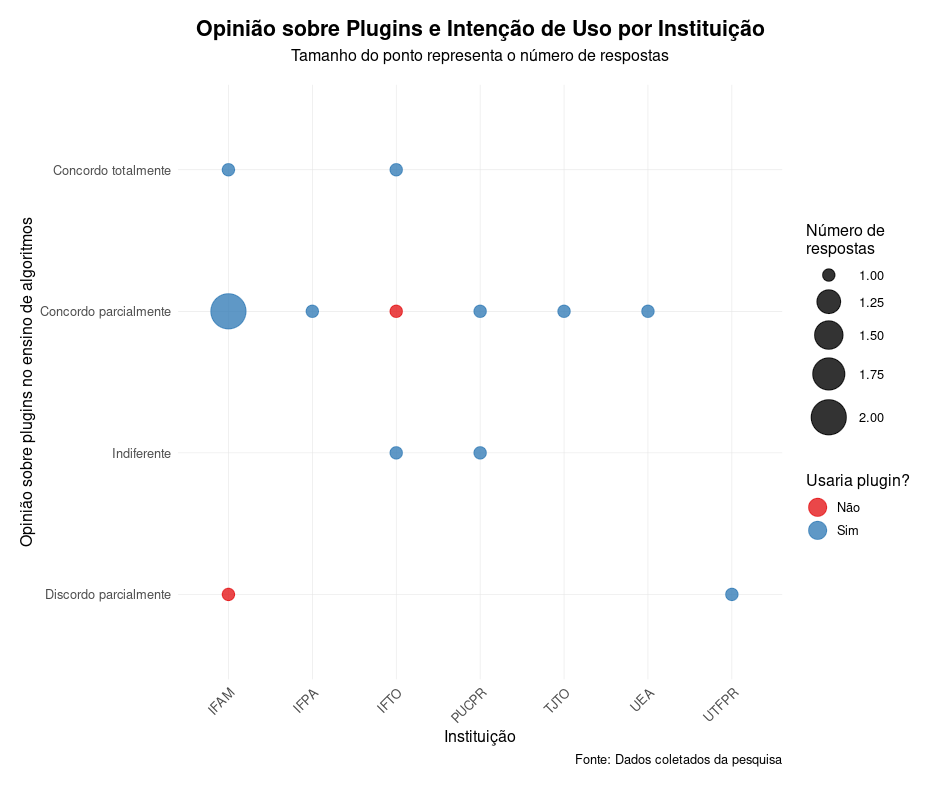
\includegraphics[width=1\linewidth]{../figuras/plugins-no-ensino-opiniao.png}
    \caption{Gráfico de pontos representando a relação entre a percepção sobre plugins educacionais e sua frequência de uso (Perguntas 9 e 11). A posição dos pontos indica a relação entre estas duas variáveis, podendo sugerir correlações.}
    \label{fig:dot-plot}
\end{figure}

A Figura \ref{fig:dot-plot} demonstra a relação entre a opinião sobre plugins no ensino e sua utilização prática. Nota-se uma tendência de avaliações mais positivas entre os usuários frequentes, sugerindo que a experiência prática influencia positivamente a percepção.

\subsection{IDEs utilizados por Instituições}
Análise de ferramentas de desenvolvimento utilizadas nas diferentes instituições. Esta visualização mostra a relação entre instituições e as IDEs utilizadas em suas aulas. Através do gráfico de barras, podemos identificar:

\begin{itemize}
    \item O Visual Studio é a IDE mais popular entre as instituições, sendo utilizadas por seis
    \item A PUCPR e UTFPR utilizam predominantemente o Visual Studio
    \item o IFAM respondeu com uma maior diversidade de IDEs
    \item Algumas instituições demonstram variedade na escolha de ferramentas
\end{itemize}
\begin{figure}[!ht]
    \centering
    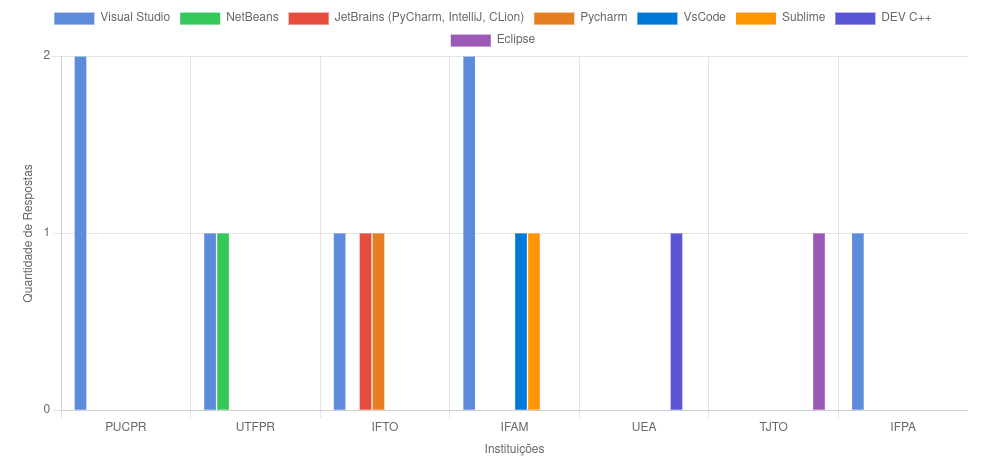
\includegraphics[width=1\linewidth]{../figuras/IDEs.png}
    \caption{Distribuição de IDEs utilizadas pelas instituições}
    \label{fig:ide}
\end{figure}